\chapter{Sampling Conformation Landscapes by Rotatable Bond Degrees of Freedom}
\label{ch:ConformationLandscape}

\section{A Brief History on Conformation Landscapes}

\subsection{Levinthal's Paradox}

In 1969, a molecular biologist by the name of Cyrus Levinthal proposed a thought experiment regarding protein formation\cite{Levinthal}:

Consider a relatively small 150-residue peptide chain completely unfolded.
This protein will have 149 peptide bonds and therefore 149 phi angles and 149 psi angles. 
Assuming three possible angle positions each, the number of possible folds of this protein follows as $3^{298}$.
How does this peptide chain fold into the appropriate secondary and tertiary structures? 
Even at attosecond rates of rotating and folding, this peptide chain would likely not fold into the correct structure for many times the age of the universe!
Obviously, this is not the case, since proteins fold on the timescale of microseconds to milliseconds.\cite{LevParadoxCalculated}
How, then, do proteins fold so quickly and efficiently?
The answer lies in energy cascades through a visualization tool called a golf course.

\subsection{Levinthal Golf Courses}

If one imagines the energy landscape of a peptide chain like a golf course, interesting similarities arise.
For example, the lowest point could be considered ``the hole" of the course with the lowest energy conformer. 
When starting at the ``tee off" point, there may not be a clean pathway of energetic difference for the ball to roll toward the global minima.
Therefore, the ball must be ``struck" toward the hole in a series of motions where the ball is removed from one local minima and placed in another hopefully closer to the hole. 
Like the image shown in figure \ref{fig:DillGC}, the course is not always an easy, natural cascade toward the global minima.
Most often, investigators will initiate several searches in several locations of this conformation landscape in hopes that one will discover a clear minima that is hopefully the true global minima.

\begin{figure}
	
	\centering
	
	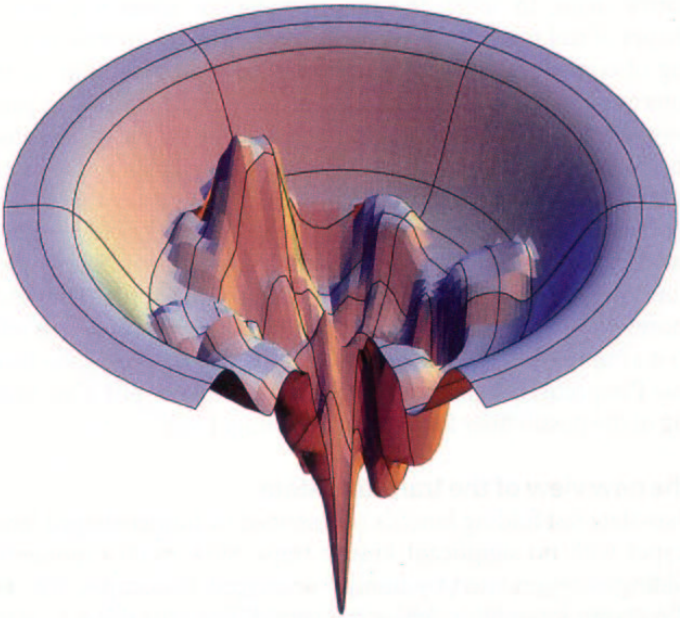
\includegraphics[width=0.75\textwidth]{DillGC.png}
	
	\caption{Example Levinthal Golf Course taken from Dill. \cite{DillLevGC}.}
	
	\label{fig:DillGC}
	
\end{figure}


\section{Purpose of Project}

As introduced in chapter \ref{ch:Germanium}, there may be a generic solution toward determining the lowest energy conformer by roughly sampling the full ``golf course" and procedurally focusing in on hot spots using automated methods.
Ideally, the tool would work through the seemingly infinite possibilities and quickly remove the impossible or duplicate conformers.
The tool would roughly take shape though a design flow detailed below.

First, the system takes an input molecule and generates a number of conformers based on rotatable dihedrals.
Second, a time-effective geometry optimization theory and basis set if necessary is selected and run files are generated and submitted to a cluster to compute.
Third, the results are collected and analyzed; low-energy dihedral values are passed back through the system while high-energy dihedrals are logged and discarded.
This restricts the conformation space to reduce the overall number of conformers generated and allows for more accurate and computationally-expensive theories and methods to calculate more reliable energies.

An overview of system flow given in figure \ref{fig:VRSDesign}.
\begin{figure}
	\centering 
	\makebox[\textwidth][c]{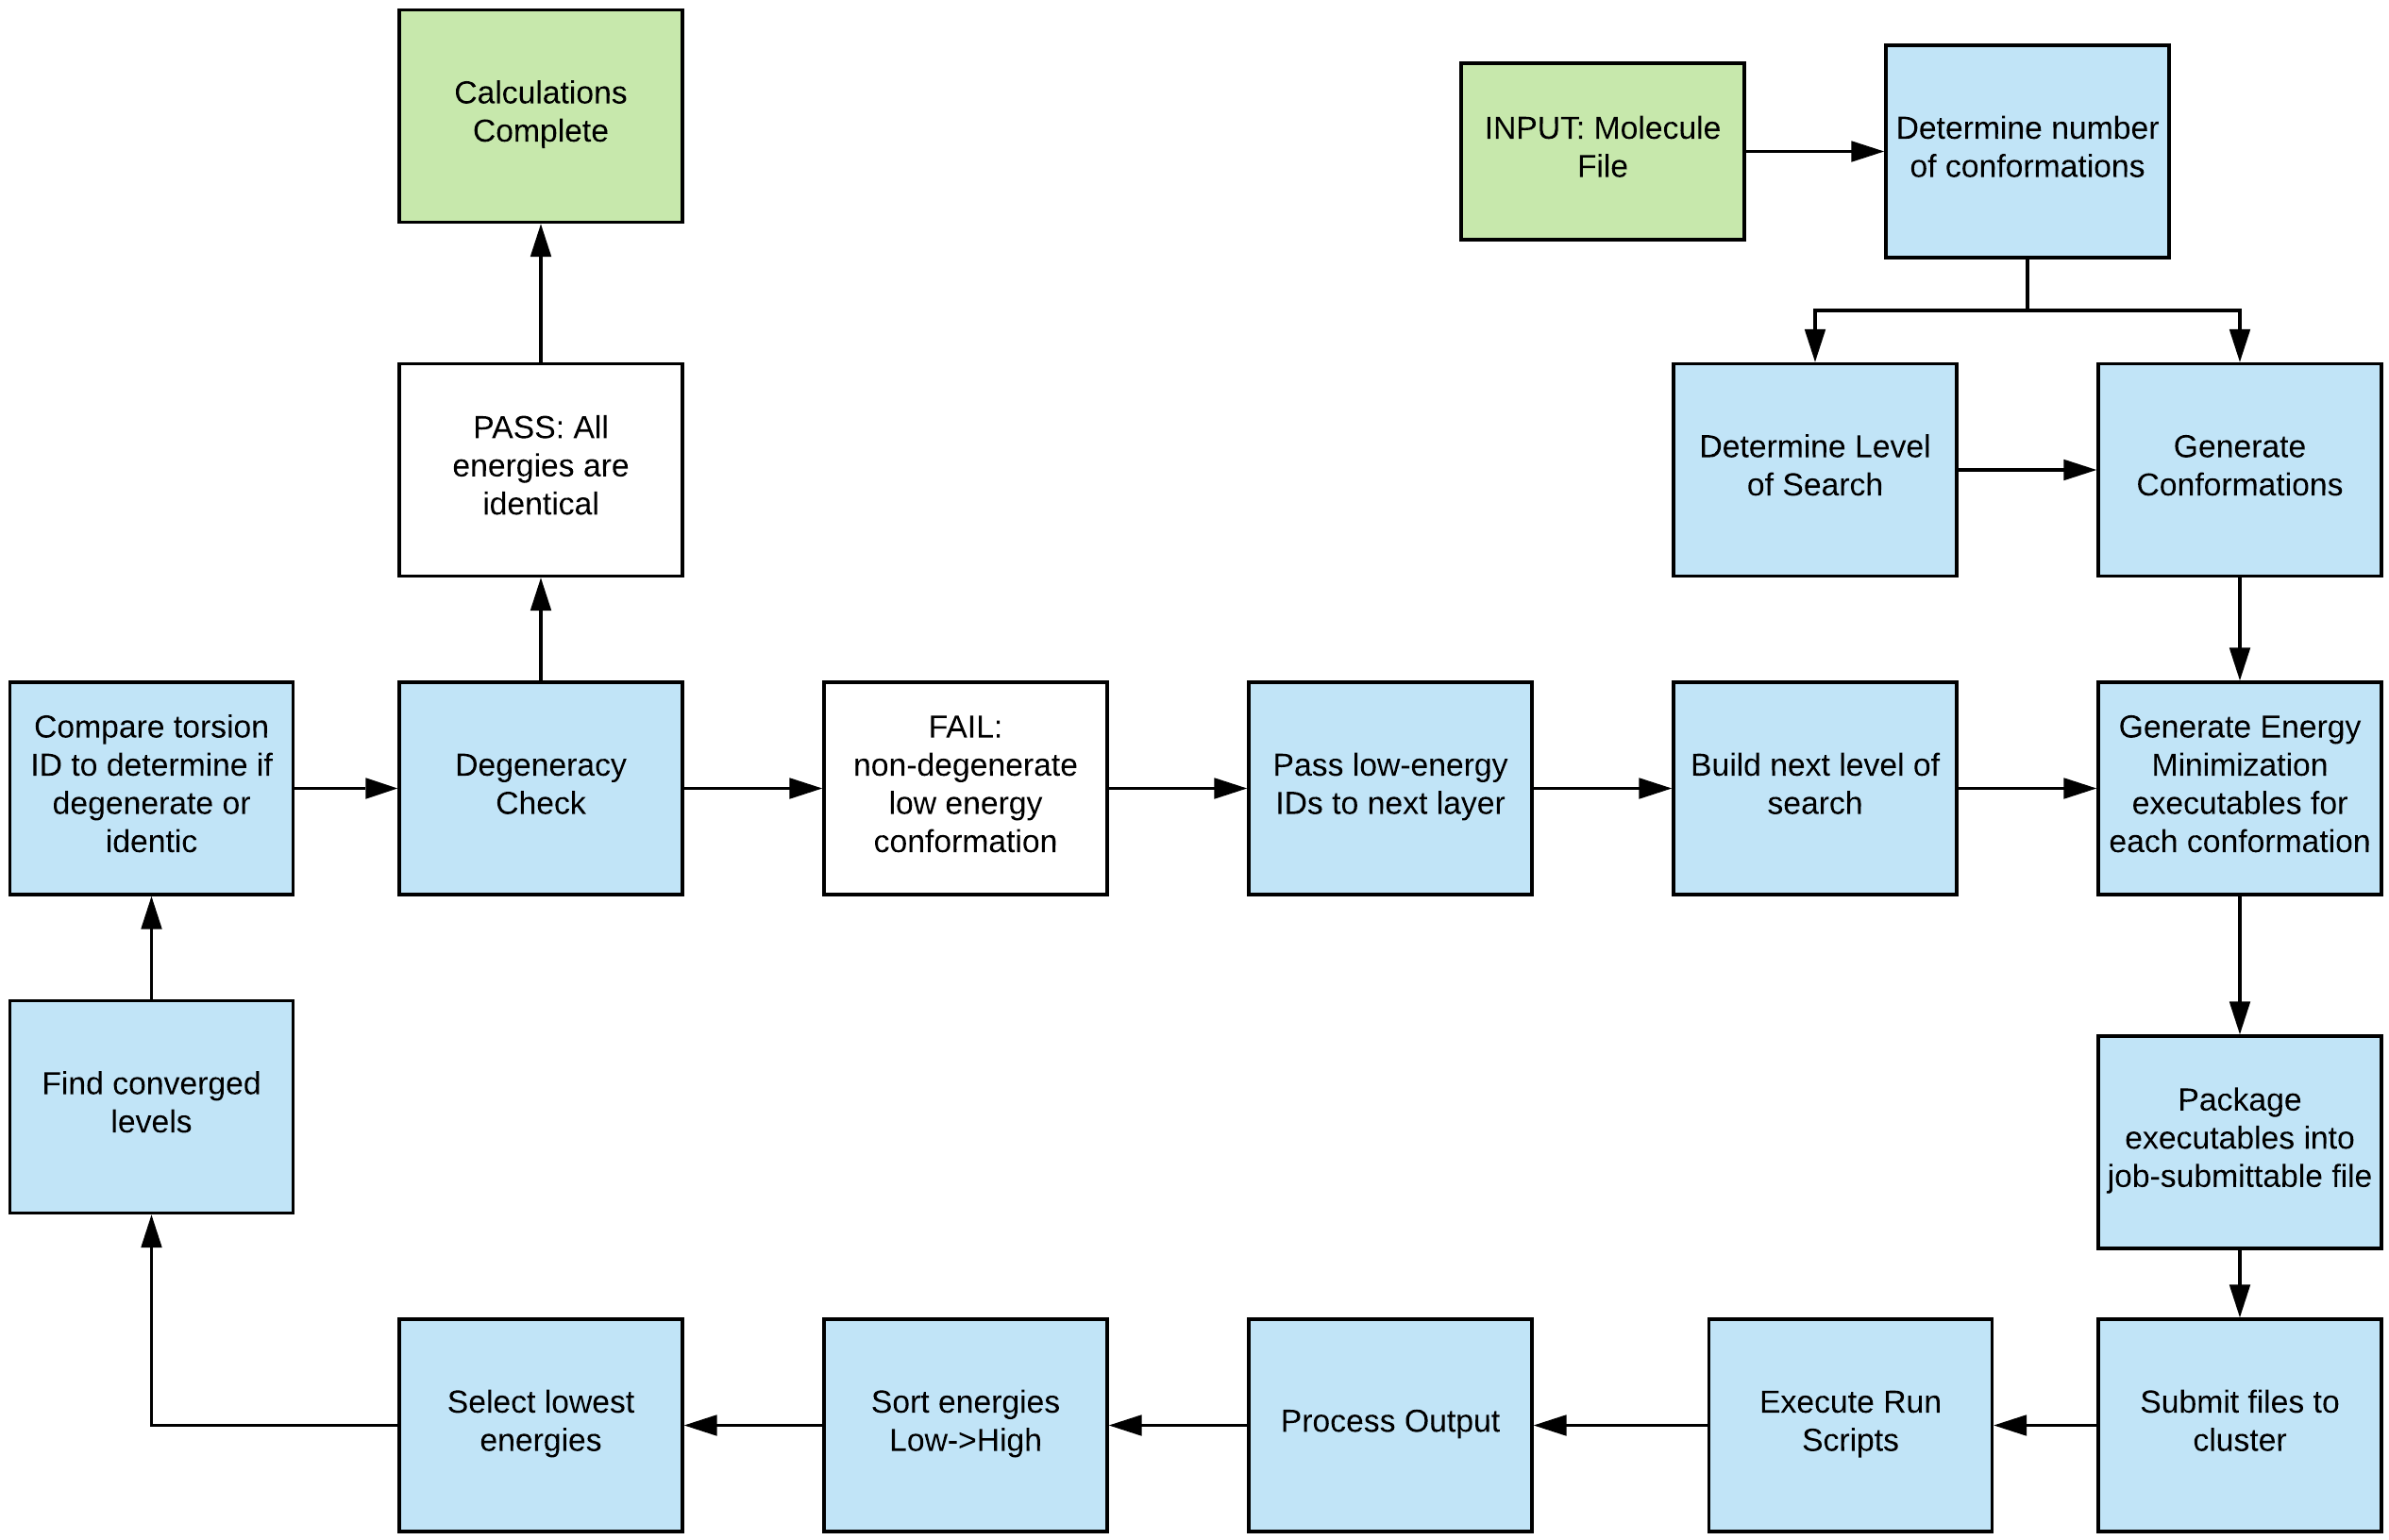
\includegraphics[width=1.3\textwidth]{AlgFlow.png}}
	\caption{Flow of method design for variable resolution conformation landscape search.}
	\label{fig:VRSDesign}
	
\end{figure}
This method produces an interesting multilayered visual plot with a zooming effect toward the lowest energy conformer.
An example of how this might look for a two-dihedral molecule is given in figure \ref{fig:variableResolutionSample}.
The outlined black boxes represent found regions of interest for future iterations of the method. 
This would repeat as necessary until regions converge to one energy.

\begin{figure}
	
	\centering
	
	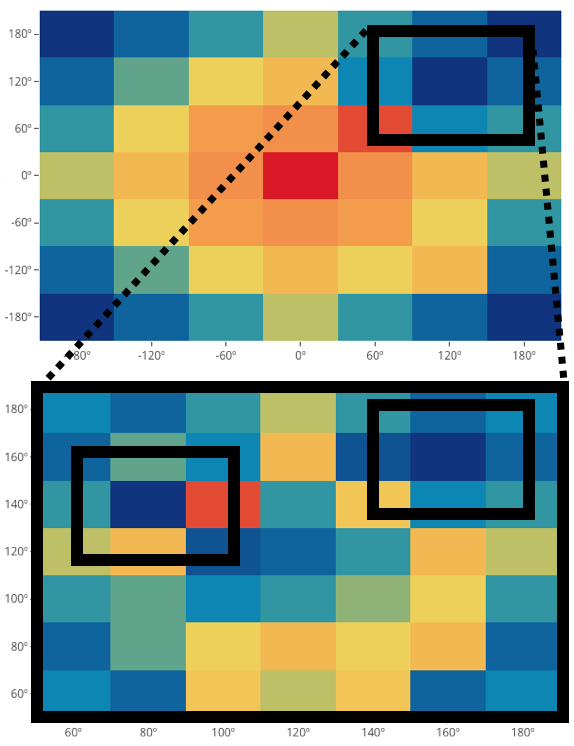
\includegraphics[width=0.75\textwidth]{VRSGraphEX.png}
	
	\caption{Example variable resolution search chart of two dihedrals with low-energy blue to high-energy red.}
	
	\label{fig:variableResolutionSample}
		
\end{figure}

\section{Design of System}

This system designed in Python for ease of development and compiled via Cython for computational efficiency. 
While it currently utilizes Gaussian 09 for energy minimization and UCSF Chimera for conformer generation, it can be redesigned for any computational programs that accomplish the desired tasks.

\subsection{Variation of Theory and Basis Set Usage by System Size and largest atom type}

Given that computational requirements increase with the number of atoms in a molecule and both the accuracy of the theory and basis set used, an initial focus on a manageable amount of conformers with a sufficiently simple theory and basis set is essential to success.
The system should estimate quantity and cost of calculations based on physcal computational constraints for various theory-basis set pairings. 
System optimizes calculation types for the scope of the landscape.
Effectively, it balances between running the first broad-scope search at relatively low accuracy and a final near-final conformation space with relatively high accuracy methods.

% Good to have: data on how theory and basis set alter computational requirement. Available in literature? Create data from runs?

\subsection{Computational Optimization by Varying Resolution}

A common problem in all works on this topic is that the scale of truly searching the conformation landscape is expansive in even the most restrictive designs. 
The manual efforts in the design of this tool are to build checkers for impossible conformations, including overlapping atom spaces.
Additional considerations are that only the most bare, three conformations per rotatable bond angle, be considered initially.
After the first round of calculations, the scope of candidates should be reduced by several orders of magnitude by refining the search about lower energy regions in the landscape.


\subsection{Inherent Complications}

The single greatest complication of this and any energy landscape tool is the number of rotatable bonds in the target molecule and, to a lesser extent, the elements contained.
Consider the hexagermane molecule of interest in chapter \ref{ch:Germanium} and the general focus of this work.
One can focus on the number of torsions available to be adjusted in the energy landscape, as shown in figure \ref{fig:Ge6Torsions}. 
Even with the minimal three rotations per bond, these 19 rotatable bonds produce $3^{19} = 1,162,261,467$ conformers, which is realistically impossible to explore even with a computational method requiring five seconds to compute.
184 years of computation time would be required.
This is where the balance between recognizing impossible conformations comes in.
Especially with bulky molecules like this hexagermane, many conformations could be eliminated by way of checking for overlapping atoms.

\begin{figure}
	\centering 
	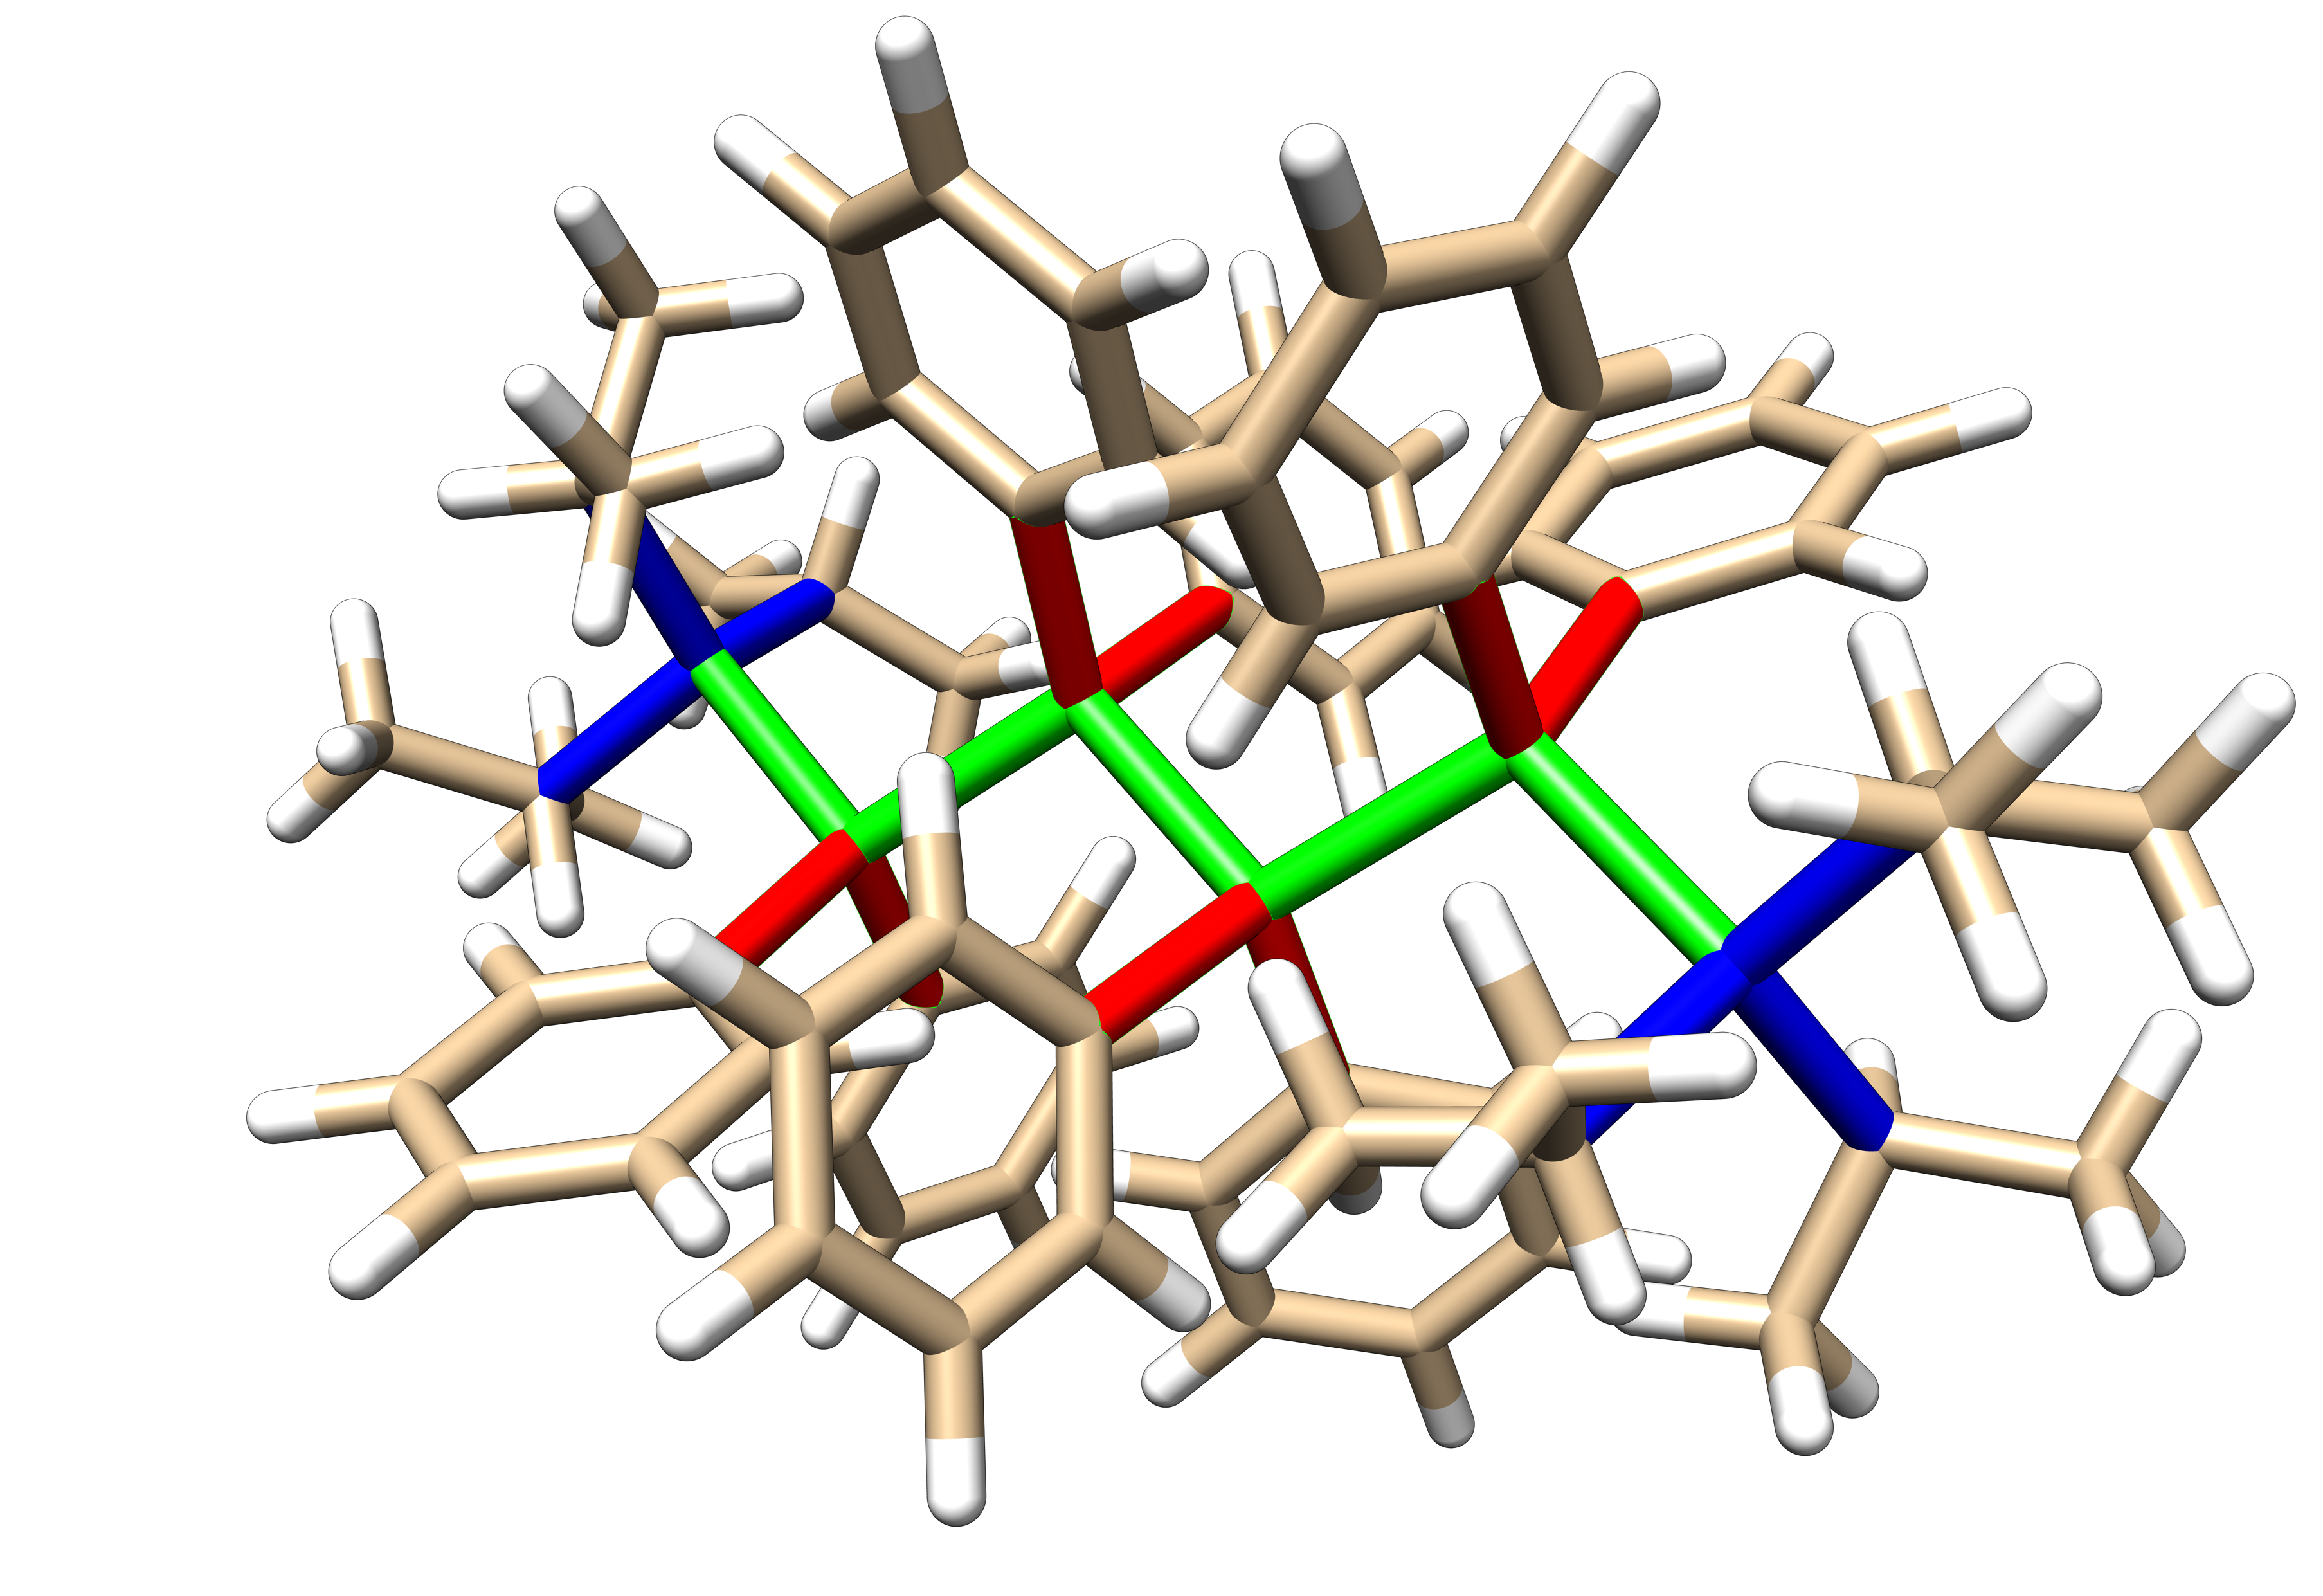
\includegraphics[width=0.75\textwidth]{Ge6Torsions.png}
	\caption{Highlighted torsions of the hexagermane molecule by type of bond, where green, red, and blue represent Ge-Ge, Ge-phenyl, and Ge-isopropyl torsion centers, respectively.}
	\label{fig:Ge6Torsions}
\end{figure}


\section{Results}

Due to the scale of the hexagermane molecule, a clear answer has not yet been discovered.
However, a much more simple run with o-nitrophenol, with only two rotatable bonds, was successful in finding the known highest and lowest energy conformer shown in figures \ref{fig:onpBad} and \ref{fig:onpGood}, respectively.

\begin{figure}
	\centering 
	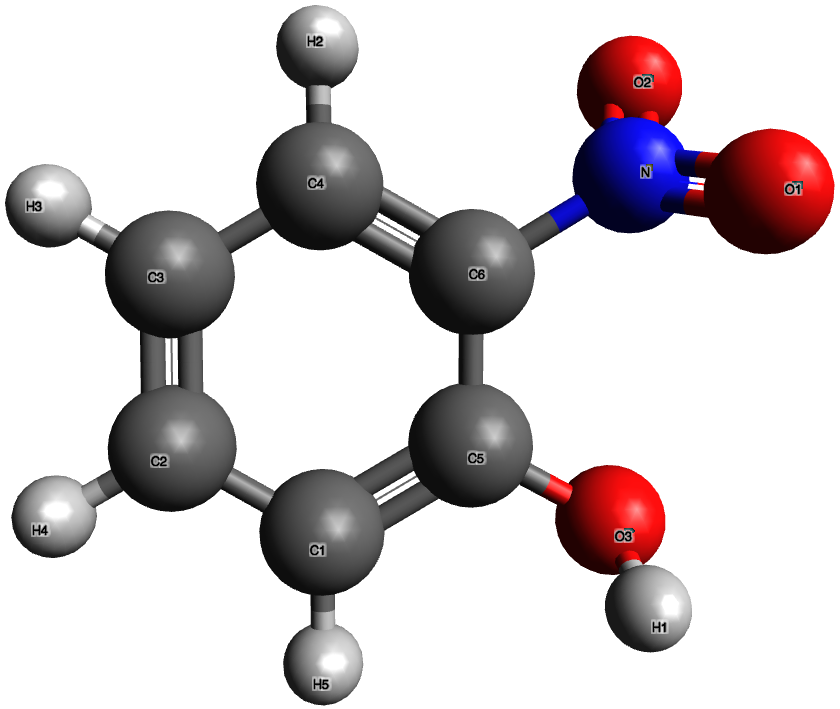
\includegraphics[width=0.75\textwidth]{onpBad.png}
	\caption{Highest energy conformer of o-nitrophenol, ignoring any ring strain conformations. This structure was notably unable to rotate and form the expected hydrogen bond between the ortho nitro and hydroxyl.}
	\label{fig:onpBad}
\end{figure}
\begin{figure}
	\centering 
	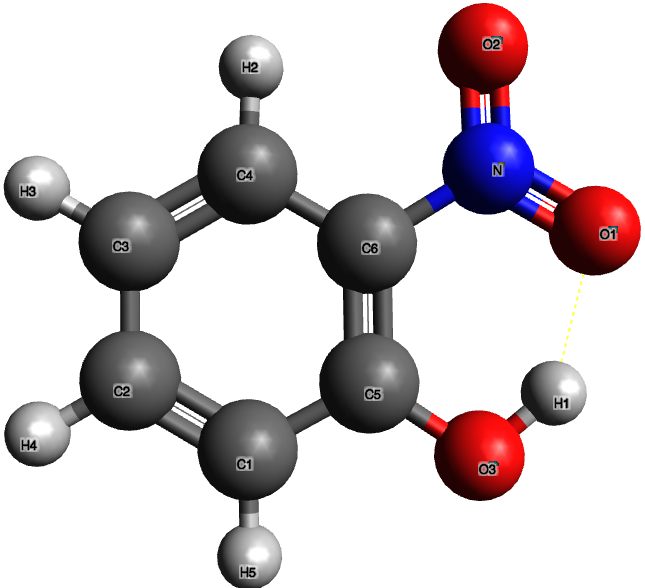
\includegraphics[width=0.75\textwidth]{onpGood.png}
	\caption{Lowest energy conformer of o-nitrophenol. Formed the expected hydrogen bond between the ortho nitro and hydroxyl.}
	\label{fig:onpGood}
\end{figure}

While these would have ideally been produced through a self-perpetuating system at increasing precisions and computation accuracy, the automated tool remains to be realized.

\subsection{Difficulties and Anticipated Future Approaches}

A key difficulty in automation of this tool is defining an abstract computation level based on arbitrary hardware limitations.
While currently limited to the Cowboy cluster at Oklahoma State University, the goal is that this tool be made available for chemists everywhere one day.
A potential solution for this abstract definition would be a small series of test runs to determine computational cost and general resource availability.

Additionally, the number of rotatable bonds yields the single largest barrier to searching the full conformation space.
With continued investigation and the inclusiveness with other works, it seems feasible that the insurmountable barrier to entry may yet be simplified in an objective way that does not prevent the system from finding the lowest energy conformer in any reasonably small molecule.
